\newpage
\def\thoigian{90}%--Thời gian
\de{Đề số 2}{Chương II. Bất phương trình và hệ bất phương trình bậc nhất hai ẩn}
% \everymath{\color{blue}}


\begin{center}
	\textbf{PHẦN 1 - CÂU TRẮC NGHIỆM BỐN PHƯƠNG ÁN}
\end{center}
\Opensolutionfile{ans}[ans/ans-TN-ONTAPCHUONG2LOP10-DE2]
%___________________________1__________________________________________
\begin{ex}%[0D2N1-1]%[Dự án dề cương 3 Khối NH24-25-Đợt 2-Nguyễn Thanh Phong]
	%THPT Phan Bội Châu Khánh Hoà 2024-2025
	Bất phương trình nào sau đây là bất phương trình bậc nhất hai ẩn?
	\choice
	{\True $-2x-3y+1<0$}
	{$2xy+3y-1 \leq 0$}
	{$3x+2y-y^3\geq 0$}
	{$-x+3y+1=0$}
	\loigiai{
		Ta thấy $-2x-3y+1<0$ là bất phương trình bậc nhất hai ẩn.
	}
\end{ex}
%============Câu 3=======================
\begin{ex}%[0D2N1-2]%[Dự án dề cương 3 Khối NH24-25-Đợt 2-Nguyễn Thanh Phong]
	Điểm nào dưới đây thuộc miền nghiệm của bất phương trình $2x - 3y \geq 7$?
	\choice
	{$M(-2; 2)$}
	{$P(4; 1)$}
	{\True $N(1; -2)$}
	{$O(0; 0)$}
	\loigiai{
		Lần lượt thay tọa độ các điểm vào bất phương trình $2x - 3y \ge 7$, ta có:
		\begin{itemize}
			\item Với điểm $M(-2; 2)$ ta được $2\cdot (-2) - 3\cdot 2 = -10 < 7$ (không thỏa mãn).
			\item Với điểm $P(4; 1)$ ta được $2\cdot 4 - 3\cdot 1 = 5 < 7$ (không thỏa mãn).
			\item Với điểm $N(1; -2)$ ta được $2 \cdot 1 - 3\cdot(-2) = 8 \geq 7$ (thỏa mãn).
			\item Với điểm $O(0; 0)$ ta được $2\cdot 0 - 3\cdot 0 = 0 < 7$ (không thỏa mãn).
		\end{itemize}
		Vậy điểm $N(1; -2)$ thuộc miền nghiệm của bất phương trình đã cho.
	}
\end{ex}
%============Câu 2=======================
\begin{ex}%[0D2H2-2]%[Dự án dề cương 3 Khối NH24-25-Đợt 2-Nguyễn Thanh Phong]
	Xét hệ bất phương trình bậc nhất hai ẩn $\heva{&2x+y \leq 2 \\ &2x+y \geq -1} \quad (1)$. Mệnh đề nào dưới đây \textbf{sai}?
	\choice
	{Tập hợp tất cả các điểm thuộc đường thẳng $d_2: 2x+y=1$ đều thuộc miền nghiệm của hệ $(1)$}
	{Tập hợp tất cả các điểm thuộc đường thẳng $d_4: 2x+y=2$ đều thuộc miền nghiệm của hệ $(1)$}
	{\True Tập hợp tất cả các điểm thuộc đường thẳng $d_3: 2x+y=-2$ đều thuộc miền nghiệm của hệ $(1)$}
	{Tập hợp tất cả các điểm thuộc đường thẳng $d_1: 2x+y=0$ đều thuộc miền nghiệm của hệ $(1)$}
	\loigiai{
		Hệ bất phương trình tương đương với $-1 \leq 2x+y \leq 2$.
		\begin{itemize}
			\item Nếu điểm thuộc đường thẳng $d_2: 2x+y=1$ thì ta có $-1 \leq 1 \leq 2$ (đúng). Vậy các điểm trên $d_2$ thuộc miền nghiệm của hệ $(1)$.
			\item Nếu điểm thuộc đường thẳng $d_4: 2x+y=2$ thì ta có $-1 \leq 2 \leq 2$ ( đúng). Vậy các điểm trên $d_4$ thuộc miền nghiệm của hệ $(1)$.
			\item Nếu điểm thuộc đường thẳng $d_3: 2x+y=-2$ thì ta có $-1 \leq -2 \leq 2$ (\textbf{sai}). Vậy các điểm trên $d_3$ không thuộc miền nghiệm của hệ $(1)$.
			\item Nếu điểm thuộc đường thẳng $d_1: 2x+y=0$ thì ta có $-1 \leq 0 \leq 2$ (đúng). Vậy các điểm trên $d_1$ thuộc miền nghiệm của hệ $(1)$.
		\end{itemize}
	}
\end{ex}

%============Câu 7=======================
\begin{ex}%[0D2N1-1]%[Dự án dề cương 3 Khối NH24-25-Đợt 2-Nguyễn Thanh Phong]
	Tìm tất cả các số thực $a$ sao cho miền nghiệm của bất phương trình $x \le a$ chứa điểm $M(-1;0)$.
	\choice
	{$a > -1$}
	{\True $a \geq -1$}
	{$a > 0$}
	{$a \geq 0$}
	\loigiai{
		Để $M(-1;0)$ thuộc miền nghiệm của bất phương trình $x \leq a$ thì $-1 \leq a$.
	}
\end{ex}
%============Câu 8=======================
\begin{ex}%[0D2H1-2]%[Dự án dề cương 3 Khối NH24-25-Đợt 2-Nguyễn Thanh Phong]
	Cho đường thẳng $d\colon 7x - 9y + 2 = 0$ chia mặt phẳng tọa độ làm hai nửa mặt phẳng. Khi đó miền nghiệm của bất phương trình $7x - 9y + 2 > 0$ là nửa mặt phẳng
	\choice
	{có chứa bờ $d$ và chứa điểm $O(0;0)$}
	{\True không chứa bờ $d$ và chứa điểm $O(0;0)$}
	{có chứa bờ $d$ và không chứa điểm $O(0;0)$}
	{không chứa bờ $d$ và không chứa điểm $O(0;0)$}
	\loigiai{
		Ta có tọa độ điểm $O(0;0)$ thỏa mãn bất phương trình $7x - 9y + 2 > 0$ nên miền nghiệm của bất phương trình $7x - 9y + 2 > 0$ là nửa mặt phẳng không có bờ $d$ và chứa điểm $O(0;0)$.
	}
\end{ex}

%============Câu 12=======================
\begin{ex}%[0D2N1-2]%[Dự án dề cương 3 Khối NH24-25-Đợt 2-Nguyễn Thanh Phong]
	Cho bất phương trình $2x+3y-2 < 0$. Miền nghiệm của bất phương trình là
	\choice
	{\True nửa mặt phẳng chứa điểm $O$ có bờ là đường thẳng $2x+3y-2=0$ (không kể bờ)}
	{nửa mặt phẳng chứa điểm $O$ có bờ là đường thẳng $2x+3y-2=0$ (kể cả bờ)}
	{nửa mặt phẳng không chứa điểm $O$ có bờ là đường thẳng $2x+3y-2=0$ (không kể bờ)}
	{nửa mặt phẳng không chứa điểm $O$ có bờ là đường thẳng $2x+3y-2=0$ (kể cả bờ)}
	\loigiai{
		Xét điểm $O(0;0)$ không thuộc đường thẳng $2x+3y-2=0$.\\
		Ta có $P = 2 \cdot 0 + 3 \cdot 0 - 2 = -2 < 0$.\\
		Vậy miền nghiệm của bất phương trình là nửa mặt phẳng chứa điểm $O$ có bờ là đường thẳng $2x+3y-2=0$ (không kể bờ).
	}
\end{ex}
%============Câu 13=======================
\begin{ex}%[0D2N1-2]%[Dự án dề cương 3 Khối NH24-25-Đợt 2-Nguyễn Thanh Phong]
	Miền nghiệm của bất phương trình $x-2y+5 < 0$ là
	\choice
	{\True Nửa mặt phẳng không chứa gốc tọa độ, bờ là đường thẳng $y = \dfrac{1}{2}x + \dfrac{5}{2}$ (không bao gồm đường thẳng)}
	{Nửa mặt phẳng chứa gốc tọa độ, bờ là đường thẳng $y = \dfrac{1}{2}x + \dfrac{5}{2}$ (không bao gồm đường thẳng)}
	{Nửa mặt phẳng không chứa gốc tọa độ, bờ là đường thẳng $y = \dfrac{1}{2}x + \dfrac{5}{2}$ (bao gồm đường thẳng)}
	{Nửa mặt phẳng chứa gốc tọa độ, bờ là đường thẳng $y = \dfrac{1}{2}x + \dfrac{5}{2}$ (bao gồm đường thẳng)}
	\loigiai{
		Xét điểm $O(0;0)$ không thuộc đường thẳng $x-2y+5=0$.\\
		Ta có $P = 1 \cdot 0 - 2 \cdot 0 +5 = 5 > 0$.\\
		Vậy miền nghiệm là nửa mặt phẳng không chứa gốc tọa độ, bờ là đường thẳng $y = \dfrac{1}{2}x + \dfrac{5}{2}$ (không bao gồm đường thẳng).
	}
\end{ex}
\begin{ex}%[0D2N2-1]%[Dự án dề cương 3 Khối NH24-25-Đợt 2-Nguyễn Thanh Phong]
	Hệ bất phương trình nào sau đây là hệ bất phương trình bậc nhất hai ẩn?
	\choice
	{$\heva{&x+\sqrt{y}>3 \\ &x-y \geq -2}$}
	{$\heva{&3x^2-20y > 7 \\ &x+y^2 \leq 100}$}
	{\True $\heva{&x>5 \\ &y+2<0}$}
	{$\heva{&x+y+z<10 \\ &x+y<5}$}
	\loigiai{Ta thấy $\heva{&x>5 \\ &y+2<0}$ là hệ bất phương trình bậc nhất hai ẩn.
	}
\end{ex}
%============Câu 4=======================
\begin{ex}%[0D2N2-2]%[Dự án dề cương 3 Khối NH24-25-Đợt 2-Nguyễn Thanh Phong]
	Cho hệ bất phương trình $\heva{&x-y<-3 \\ &7x+2y \geq 1}$. Điểm nào sau đây thuộc miền nghiệm của hệ đã cho?
	\choice
	{$(-3;1)$}
	{\True $(0;5)$}
	{$(2;1)$}
	{$(-2;-5)$}
	\loigiai{Ta đặt hệ bất phương trình $\heva{&x-y<-3 \\ &7x+2y \geq 1}$ $(*)$.
		\begin{itemize}
			\item Thay $(-3;1)$ vào $(*)$ ta được $\heva{&-4<-3 \\ &-19 \geq 1}$. Do đó điểm $(-3;1)$ không thoả $(*)$.
			\item Thay $(0;5)$ vào $(*)$ ta được $\heva{&-5<-3 \\ &10 \geq 1}$. Do đó điểm $(0;5)$ thoả $(*)$.
			\item Thay $(2;1)$ vào $(*)$ ta được $\heva{&1<-3 \\ &16 \geq 1}$. Do đó điểm $(2;1)$ không thoả $(*)$.
			\item Thay $(-2;-5)$ vào $(*)$ ta được $\heva{&3<-3 \\ &-24 \geq 1}$. Do đó điểm $(-2;-5)$ không thoả $(*)$.
		\end{itemize}
	}
\end{ex}
%============Câu 5=======================
\begin{ex}%[0D2H2-2]%[Dự án dề cương 3 Khối NH24-25-Đợt 2-Nguyễn4 Thanh Phong]
	Phần không tô màu ở hình bên dưới (không kể bờ) là biểu diễn miền nghiệm của hệ bất phương trình nào sau đây?
	\begin{center}
		\begin{tikzpicture}[scale=1,font=\footnotesize,line join=round,line cap=round,>=stealth]
			\def\xmin{-1} \def\xmax{4.5}
			\def\ymin{-2} \def\ymax{4.6}
			\fill[gray!60] (\xmin, \ymin) rectangle (\xmax, 0);
			\begin{scope}
				\clip (\xmin, 0) rectangle (\xmax, \ymax);
				\fill[pattern=dots, pattern color=black!70]
				(\xmin, {-1.5*(\xmin)+3}) -- plot[domain=\xmin:\xmax] (\x, {-1.5*(\x)+3})
				-- (\xmax, \ymax) -- (\xmin, \ymax) -- cycle;
			\end{scope}
			\draw[->] (\xmin,0) -- (\xmax,0) node[right] {$x$};
			\draw[->] (0,\ymin) -- (0,\ymax) node[above] {$y$};
			\draw[thick, black, domain=\xmin:\xmax-1.2]
			plot(\x, {-1.5*(\x)+3})
			node[pos=0.45, sloped,yshift=1.2cm,xshift=0.8cm, rotate=-55] {$3x+2y-6=0$};
			\node[below=2pt] at (2,0) {2};
			\node[left=2pt] at (0,3) {3};
			\node[below left, inner sep=1pt] at (0,0) {$O$};
		\end{tikzpicture}	
	\end{center}
	\choice
	{\True $\heva{&y>0 \\&3x+2y < 6}$}
	{$\heva{&y>0 \\ &3x+2y < -6}$}
	{$\heva{&x>0 \\ &3x+2y < 6}$}
	{$\heva{&x>0 \\& 3x+2y > -6}$}
	\loigiai{
		Miền không tô màu biểu diễn miền nghiệm $\heva{&y>0 \\&3x+2y < 6.}$
	}
\end{ex}
%============Câu 7=======================
\begin{ex}%[0D2N2-2]%[Dự án dề cương 3 Khối NH24-25-Đợt 2-Nguyễn Thanh Phong]
	Cặp số nào sau đây \textbf{không} là một nghiệm của hệ bất phương trình $\heva{&x+y \leq 2 \\&2x-3y > -2}$?
	\choice
	{$(0;0)$}
	{$(1;1)$}
	{\True $(-1;1)$}
	{$(-1;-1)$}
	\loigiai{
		\begin{itemize}
			\item Thay $(0;0)$ vào hệ bất phương trình trên, ta được: $\heva{&0\leq 2 \\&0>-2}$. Do đó $(0;0)$ là nghiệm của hệ bất phương trình trên.
			\item Thay $(1;1)$ vào hệ bất phương trình trên, ta được: $\heva{&2\leq 2 \\&-1>-2}$. Do đó $(1;1)$ là nghiệm của hệ bất phương trình trên.
			\item Thay $(-1;1)$ vào hệ bất phương trình trên, ta được: $\heva{&0\leq 2 \\&-5>-2}$. Do đó $(-1;1)$ là không nghiệm của hệ bất phương trình trên.
			\item Thay $(-1;-1)$ vào hệ bất phương trình trên, ta được: $\heva{&-2\leq 2 \\&1>-2}$. Do đó $(1;1)$ là nghiệm của hệ bất phương trình trên.
		\end{itemize}
	}
\end{ex}

\begin{ex}%[0D2V2-3]%[Dự án dề cương 3 Khối NH24-25-Đợt 2-Nguyễn Thanh Phong]
	Một cửa hàng dự định kinh doanh hai loại máy điều hòa: điều hòa một chiều và điều hòa hai chiều. Khảo sát thị trường của hàng thấy nhu cầu của thị trường sẽ không vượt quá $100$ máy cả hai loại. Gọi $x$, $y$ lần lượt là số máy điều hòa một chiều và điều hòa hai chiều mà cửa hàng nhập vào. Khi đó, $(x; y)$ là nghiệm của hệ bất phương trình nào dưới đây?
	\choice
	{\True $\heva{&x \geq 0 \\ &y \geq 0 \\ &x+y \leq 100}$}
	{$\heva{&x \geq 0 \\& y \geq 0 \\& x+y < 100}$}
	{$\heva{&x \geq 0 \\& y \geq 0 \\& x+y \geq 100}$}
	{$\heva{&x \geq 0 \\& y \geq 0 \\& x+y > 100}$}
	\loigiai{
		Giả thiết cho $x$, $y$ lần lượt là số lượng máy điều hoà một chiều và điều hoà hai chiều $(x, \; y \geq 0)$.\\
		Vì nhu cầu của thị trường sẽ không vượt quá $100$ máy cả hai loại nên $x+y \leq 100$.\\
		Vậy $\heva{&x \geq 0 \\ &y \geq 0 \\ &x+y \leq 100.}$
	}
\end{ex}
\Closesolutionfile{ans}
%\begin{center}
%	\textbf{ĐÁP ÁN}
%	\inputansbox{10}{ans/ans}	
%\end{center}


\setcounter{ex}{0}
\begin{center}
	\textbf{PHẦN 2 - CÂU TRẮC NGHIỆM ĐÚNG SAI}
\end{center}

\Opensolutionfile{ans}[ans/answer-DS-ONTAPCHUONG2LOP10-DE2]
%============Câu 1=======================
\begin{ex}%[0D2N1-2]%[Dự án dề cương 3 Khối NH24-25-Đợt 2-Nguyễn Thanh Phong]
	Cho điểm $(-1;2)$ và các bất phương trình $3x-5y < -15$, $2x+y \leq 0$, $3x-9y > 7$, $-4x+3y \geq 5$. Khi đó
	\choiceTF
	{\True $(-1;2)$ \textbf{không} là một nghiệm của bất phương trình $3x-5y < -15$}
	{\True $(-1;2)$ là một nghiệm của bất phương trình $2x+y \leq 0$}
	{$(-1;2)$ là một nghiệm của bất phương trình $3x-9y > 7$}
	{\True $(-1;2)$ là một nghiệm của bất phương trình $-4x+3y \geq 5$}
	\loigiai{
		\begin{itemchoice}
			\itemch \textbf{Đúng.} Thay $(-1;2)$ vào bất phương trình $3x-5y < -15$, ta được $-13 > -15$ nên $(-1;2)$ không là nghiệm của bất phương trình này.
			\itemch \textbf{Đúng.} Thay $(-1;2)$ vào bất phương trình $2x+y \leq 0$, ta được $0 \leq 0$ nên $(-1;2)$ là nghiệm của bất phương trình này.
			\itemch \textbf{Sai.} Thay $(-1;2)$ vào bất phương trình $3x-9y > 7$, ta được $-21 > 7$ nên $(-1;2)$ không là nghiệm của bất phương trình này.
			\itemch \textbf{Đúng} Thay $(-1;2)$ vào bất phương trình $-4x+3y \geq 5$, ta được $10 \geq 5$ nên $(-1;2)$ là nghiệm của bất phương trình này. 
		\end{itemchoice}
	}
\end{ex}
%============Câu 2=======================
\begin{ex}%[0D2V2-3]%[Dự án dề cương 3 Khối NH24-25-Đợt 2-Nguyễn Thanh Phong]
	Bác An dự định trồng hai loại cây là cà phê và tiêu trong nông trại rộng $30$ héc-ta. Biết mỗi héc-ta trồng cà phê cần $20$ công chăm sóc và thu lợi nhuận $200$ triệu đồng, mỗi héc-ta trồng tiêu cần $40$ công chăm sóc và thu lại lợi nhuận $180$ triệu đồng. Biết rằng tổng số công cần dùng không được vượt quá $800$ công. Gọi $x$ và $y$ (héc-ta) lần lượt diện tích đất dùng để trồng cà phê và tiêu.
	\choiceTF
	{\True Số công cần dùng để sản xuất $x$ héc-ta cà phê và $y$ héc-ta tiêu thoả mãn bất phương trình $x+2y \leq 40$}
	{\True Lợi nhuận thu được khi sản xuất $x$ héc-ta cà phê và $y$ héc-ta tiêu là $200x+180y$ (triệu đồng)}
	{Miền nghiệm của hệ bất phương trình $\heva{&x \geq 0 \\&y \geq 0 \\&x+y \leq 30 \\&x+2y \leq 40}$ là một đa giác có diện tích bằng $400$ (đvdt)}
	{Lợi nhuận cao nhất mà bác An có thể thu được là $5{,}8$ tỉ đồng}
	\loigiai{
		\begin{itemchoice}
			\itemch \textbf{Đúng.} Số công cần dùng để sản xuất $x$ héc-ta cà phê và $y$ héc-ta tiêu là $20x+40y \leq 800 \Rightarrow x+2y \leq 40$.
			\itemch \textbf{Đúng.} Lợi nhuận thu được khi sản xuất $x$ héc-ta cà phê và $y$ héc-ta tiêu là $200x+180y$ (triệu đồng).
			\itemch \textbf{Sai.}
			\begin{center} 
				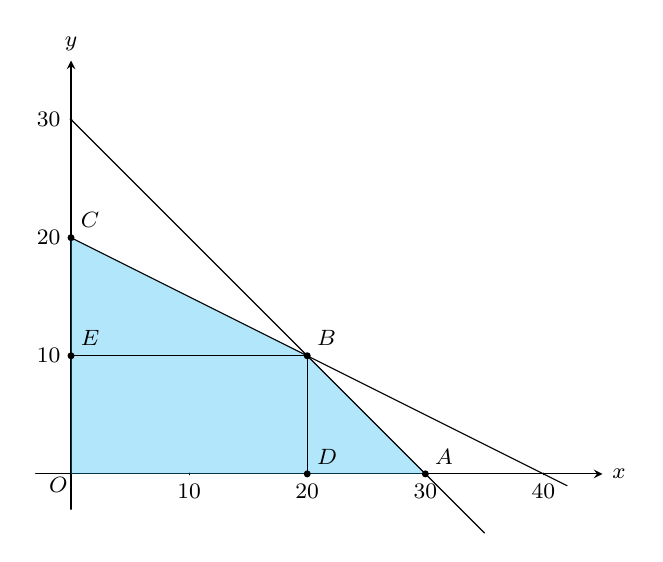
\begin{tikzpicture}[scale=0.15,font=\footnotesize,line join=round,line cap=round,>=stealth]
					\def\xmin{-3} \def\xmax{45} \def\ymin{-3} \def\ymax{35}
					\draw[->] (\xmin,0) -- (\xmax,0) node[right] {$x$};
					\draw[->] (0,\ymin) -- (0,\ymax) node[above] {$y$};
					\foreach \val in {10,20,30,40} \draw(\val,2pt)--(\val,-2pt) node[below]{$\val$};
					\foreach \val in {10,20,30} \draw(2pt,\val)--(-2pt,\val) node[left]{$\val$};
					\node[below left,inner sep=1pt] at (0,0){$O$};
					\coordinate (O) at (0,0);
					\coordinate (A) at (30,0);
					\coordinate (B) at (20,10);
					\coordinate (C) at (0,20);
					\fill[cyan,opacity=0.3] (O)--(A)--(B)--(C)--cycle;
					\draw[domain=0:35] plot(\x,{30-\x});
					\draw[domain=0:42] plot(\x,{20-0.5*\x});
					\draw (0,10)--(20,10) (20,0)--(20,10);
					\filldraw (0,10) circle (7pt) node[above right]{$E$};
					\filldraw (B) circle (7pt) node[above right]{$B$};
					\filldraw (20,0) circle (7pt) node[above right]{$D$};
					\filldraw (C) circle (7pt) node[above right]{$C$};
					\filldraw (A) circle (7pt) node[above right]{$A$};
				\end{tikzpicture}
			\end{center}
			Ta vẽ miền nghiệm của hệ bất phương trình $\heva{&x \geq 0 \\&y \geq 0 \\&x+y \leq 30 \\&x+2y \leq 40}$ và chia miền thành các $\triangle CEB$, $\triangle ABD$ và tứ giác $OEBD$. Khi đó, ta tính:
			\begin{align*}
				\triangle CEB &= \dfrac{1}{2}\cdot EB \cdot CE=\dfrac{1}{2}\cdot 20 \cdot 10=100. \\
				\triangle ABD &= \dfrac{1}{2}\cdot AD \cdot BD=\dfrac{1}{2}\cdot 10 \cdot 10 =50.\\
				OEBD &= OD \cdot OE = 20 \cdot 10 = 200.
			\end{align*}
			Diện tích của miền nghiệm: $100+50+200=350$ (đvdt).
			\itemch \textbf{Sai.} Từ miền nghiệm, ta có bảng sau:
			\begin{center}
				\begin{tabular}{c|c|c|c|c}
					& $O$ & $A$ & $B$ & $C$ \\
					\hline 
					$(x;y)$ & $(0;0)$ & $(30;0)$ & $(20;10)$ & $(0;20)$ \\
					\hline 
					$200x+180y$ & $0$ & $6\,000$ & $5\,800$ & $3\,600$ 
				\end{tabular}
			\end{center}
			Từ bảng, lợi nhuận cao nhất mà bác An thu được là $6\,000$ triệu đồng hay $6$ tỷ đồng.
		\end{itemchoice}
	}
\end{ex}

%============Câu 2=======================

\Closesolutionfile{ans}
%\inputansbox[2]{2}{ans/answer.tex}



\begin{center}
	\textbf{PHẦN 3 - CÂU TRẮC NGHIỆM TRẢ LỜI NGẮN}
\end{center}
\setcounter{ex}{0}
\Opensolutionfile{ans}[ans-KQ-ONTAPCHUONG2LOP10-DE2]

%============Câu 1=======================
\begin{ex}%[0D2V1-3]%[Dự án dề cương 3 Khối NH24-25-Đợt 2-Nguyễn Thanh Phong]
	Có bao nhiêu nghiệm $(x,y)$ của bất phương trình $\dfrac{x}{2}+\dfrac{y}{3}-1 \leq 0$ thỏa mãn $x$, $y$ là các số nguyên dương.
	\par\shortans[]{$1$}
	\loigiai{
		Bất phương trình $\dfrac{x}{2}+\dfrac{y}{3}-1 \leq 0$ tương đương với $3x+2y\leq 6$.\\
		Khi đó, chỉ có $1$ cặp $(x,y)$ nguyên dương thoả mãn bất phương trình là $(1;1)$.
	}
\end{ex}

%============Câu 2=======================
\begin{ex}%[0D2H1-1]%[Dự án dề cương 3 Khối NH24-25-Đợt 2-Nguyễn Thanh Phong]
	Cho bất phương trình $2x - (m+2)y + m \leq 0$. Có bao nhiêu giá trị nguyên âm của tham số $m$ để bất phương trình có một nghiệm là $(1;3)$.
	\par\shortans[]{$2$}
	\loigiai{
		Thay $(1;3)$ và bất phương trình trên, ta được: 
		\begin{eqnarray*}
			&&2-(m+2)\cdot 3+m \leq 0\\
			\Rightarrow& &2-3m-6+m\leq 0 \\
			\Rightarrow& &-2m -4 \leq 0 \\
			\Rightarrow& &m \geq -2. 
		\end{eqnarray*}
		Ta chỉ nhận giá trị nguyên âm của $m$ nên $m \in \{-2;-1\}$.\\
		Vậy có $2$ giá trị nguyên âm của $m$ thoả yêu cầu bài toán.
	}
\end{ex}
%============Câu 4=======================
\begin{ex}%[0D2V2-3]%[Dự án dề cương 3 Khối NH24-25-Đợt 2-Nguyễn Thanh Phong]
	Tìm giá trị lớn nhất của biểu thức $F(x;y)=3y-2x$ với $(x;y)$ là nghiệm của hệ bất phương trình:
	$\heva{&x-10y \leq 35 \\&x-y \geq -1 \\&2x+y \leq 7}$ có miền nghiệm là miền tam giác $ABC$ như hình vẽ dưới đây
	\begin{center}
		\begin{tikzpicture}[scale=0.7,font=\footnotesize,line join=round,line cap=round,>=stealth]
			\def\xmin{-6} \def\xmax{7} \def\ymin{-5} \def\ymax{5}
			\coordinate (A) at (5,-3);
			\coordinate (B) at (2,3);
			\coordinate (C) at (-5,-4);
			\draw[->] (\xmin,0) -- (\xmax,0) node[right] {$x$};
			\draw[->] (0,\ymin) -- (0,\ymax) node[above] {$y$};
			\foreach \pos/\lab in {-5/-5, 2/2, 5/5}
			\draw (\pos,1.5pt) -- (\pos,-1.5pt) node[below] {$\lab$};
			\foreach \pos/\lab in {-4/-4, -3/-3, 3/3}
			\draw (1.5pt,\pos) -- (-1.5pt,\pos) node[left] {$\lab$};
			\node[below right, inner sep=1pt] at (0,0) {$O$};
			\begin{scope}
				\clip (-6,-5) -- (B) -- (\xmax,\ymax) -- (\xmin-1,\ymax) -- cycle;
				\fill[pattern=north west lines, pattern color=brown, opacity=0.7] (\xmin,\ymin) rectangle (\xmax,\ymax);
			\end{scope}
			\begin{scope}
				\clip (A) -- (B) -- (\xmax,\ymax) -- (\xmax,\ymin) -- cycle;
				\fill[pattern=north west lines, pattern color=green!60!black, opacity=0.7] (\xmin,\ymin) rectangle (\xmax,\ymax);
			\end{scope}
			\begin{scope}
				\clip (C) -- (A) -- (\xmax,\ymin) -- (\xmin,\ymin) -- cycle;
				\fill[pattern=north west lines, pattern color=blue, opacity=0.7] (\xmin,\ymin) rectangle (\xmax,\ymax);
			\end{scope}
			% \draw[dashed] (A) -- (5,0) (A) -- (0,-3);
			\draw[dashed] (B) -- (2,0) (B) -- (0,3);
			% \draw[dashed] (C) -- (-5,0) (C) -- (0,-4);
			\clip (\xmin, \ymin) rectangle (\xmax, \ymax);
			\draw[thick, blue!50!black, domain=\xmin:\xmax, samples=2] plot(\x, {-2*\x+7}); 
			\draw[thick, purple, domain=\xmin:\xmax, samples=2] plot(\x, {\x+1}); 
			\draw[thick, blue!50!black, domain=\xmin:\xmax, samples=2] plot(\x, {0.1*\x-3.5});
			\fill (A) circle (1.5pt) node[right,yshift=-3pt] {$A$};
			\fill (B) circle (1.5pt) node[above, yshift=2pt] {$B$};
			\fill (C) circle (1.5pt) node[below right] {$C$};
		\end{tikzpicture}
	\end{center}
	\par\shortans[]{$5$}
	\loigiai{
		Miền nghiệm của hệ bất phương trình là miền tam giác $ABC$ với các đỉnh là giao điểm của các đường thẳng tương ứng: $d_1\colon x-10y = 35$; $d_2\colon x-y = -1$; $d_3\colon 2x+y = 7$.
		\begin{itemize}
			\item Tọa độ điểm $A$ là nghiệm của hệ $\heva{&x-10y = 35 \\&2x+y = 7} \Rightarrow \heva{&x=5 \\&y=-3.}$ Vậy $A(5; -3)$.
			\item Tọa độ điểm $B$ là nghiệm của hệ $\heva{&x-y = -1 \\&2x+y = 7} \Rightarrow \heva{&x=2 \\&y=3.}$ Vậy $B(2; 3)$.
			\item Tọa độ điểm $C$ là nghiệm của hệ $\heva{&x-10y = 35 \\&x-y = -1} \Rightarrow \heva{&x=-5 \\&y=-4.}$ Vậy $C(-5; -4)$.
		\end{itemize}
		Giá trị lớn nhất của biểu thức $F(x;y)=3y-2x$ trên miền tam giác $ABC$ đạt được tại đỉnh của tam giác. Ta tính giá trị của $F$ tại các đỉnh:
		\begin{itemize}
			\item $F(5; -3) = 3\cdot (-3) - 2 \cdot 5 = -9 - 10 = -19$.
			\item $F(2; 3) = 3\cdot 3 - 2\cdot 2 = 9 - 4 = 5$.
			\item $F(-5; -4) = 3\cdot (-4) - 2\cdot (-5) = -12 + 10 = -2$.
		\end{itemize}
		So sánh các giá trị, ta thấy giá trị lớn nhất của $F(x;y)$ là $5$, đạt được tại điểm $B(2; 3)$.
	}
\end{ex}

\begin{ex}%[0D2V2-3]%[Dự án dề cương 3 Khối NH24-25-Đợt 2-Nguyễn Thanh Phong]
	Đợt cuối năm, do nhu cầu tiêu dùng tăng cao, một cửa hàng kinh doanh xe máy dự định kinh doanh bổ sung hai loại xe máy của Honda là xe máy Lead và xe máy Vision, với số vốn ban đầu không vượt quá $36$ tỉ đồng. Giá nhập về một chiếc xe máy Lead là $40$ triệu đồng, lợi nhuận dự kiến là $5$ triệu đồng một chiếc. Giá nhập về một chiếc xe máy Vision là $30$ triệu đồng, lợi nhuận dự kiến là $3{,}2$ triệu đồng một chiếc. Cửa hàng ước tính rằng tổng nhu cầu thị trường không vượt quá $1100$ chiếc xe cả hai loại và nhu cầu xe Lead không vượt quá $1{,}5$ lần nhu cầu xe Vision. Hỏi lợi nhuận có thể thu được lớn nhất của cửa hàng là bao nhiêu tiền?
	\par\shortans[]{$4\,280$}
	\loigiai{
		Gọi $x$, $y$ lần lượt là số lượng xe máy Lead và xe máy Vision $(x$, $y \in \mathbb{N})$. Khi đó:
		\begin{itemize}
			\item Số tiền để nhập hai loại xe về không quá $36$ tỉ đồng nên $40x+30y \leq 36\,000 \Rightarrow 4x+3y \leq 3\,600$.
			\item Nhu cầu thị trường không vượt quá $1100$ xe cả $2$ loại nên $x+y \leq 1100$.
			\item Nhu cầu xe Lead không vượt quá $1{,}5$ lần xe Vision nên $x \leq 1{,5}y \Rightarrow x-1{,}5y \leq 0$.
			\item Lợi nhuận khi bán hai loại xe trên: $5x+3{,}2y$ (triệu đồng).
		\end{itemize} 
		\begin{center}
			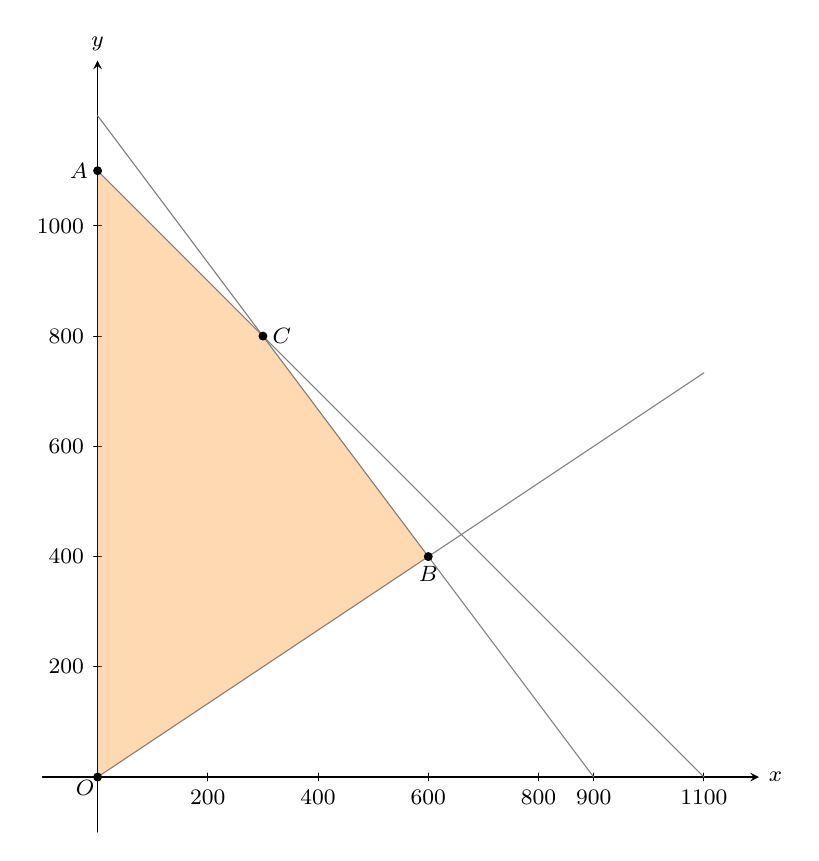
\begin{tikzpicture}[scale=0.7,font=\footnotesize,line join=round,line cap=round,>=stealth]
				\def\xmin{-1} \def\xmax{12} \def\ymin{-1} \def\ymax{13}
				\draw[->] (\xmin,0) -- (\xmax,0) node[right] {$x$};
				\draw[->] (0,\ymin) -- (0,\ymax) node[above] {$y$};
				\draw (2,2pt)--(2,-2pt) node[below]{$200$};
				\draw (4,2pt)--(4,-2pt) node[below]{$400$};
				\draw (6,2pt)--(6,-2pt) node[below]{$600$};
				\draw (8,2pt)--(8,-2pt) node[below]{$800$};
				\draw (9,2pt)--(9,-2pt) node[below]{$900$};
				\draw (11,2pt)--(11,-2pt) node[below]{$1100$};
				\draw (2pt,2)--(-2pt,2) node[left]{$200$};
				\draw (2pt,4)--(-2pt,4) node[left]{$400$};
				\draw (2pt,6)--(-2pt,6) node[left]{$600$};
				\draw (2pt,8)--(-2pt,8) node[left]{$800$};
				\draw (2pt,10)--(-2pt,10) node[left]{$1000$};
				
				\node[below left, inner sep=1pt] at (0,0){$O$};
				\coordinate (O) at (0,0);
				\coordinate (A) at (0,11);
				\coordinate (B) at (3,8);
				\coordinate (C) at (6,4);
				\fill[orange,opacity=0.3] (O)--(A)--(B)--(C)--cycle;
				\draw[gray,domain=0:9] plot(\x,{12-(4/3)*\x});
				\draw[gray,domain=0:11] plot(\x,{11-\x});
				\draw[gray,domain=0:11] plot(\x,{(2/3)*\x});
				\filldraw (0,0) circle (2pt);
				\filldraw (0,11) circle (2pt)node[left]{$A$};
				\filldraw (6,4) circle (2pt)node[below]{$B$};
				\filldraw (3,8) circle (2pt)node[right]{$C$};
			\end{tikzpicture}
		\end{center}
		Ta kí hiệu các điểm $A$, $B$, $C$ như hình. Trong đó $C$ là giao điểm giữa hai đường thẳng $x+y=1100$ và $4x+3y=3600$. Khi đó:
		$$\heva{&x+y=1100\\&4x+3y=3600}\Rightarrow \heva{&x=300\\&y=800} \Rightarrow C(300;800).$$
		Từ miền nghiệm của bài toán, ta có bảng sau:
		\begin{center}
			\begin{tabular}{c|c|c|c|c}
				&$O$ &$A$ &$B$& $C$   \\ 
				\hline 
				$(x;y)$ &$(0;0)$ & $(0;1100)$ & $(600;400)$ & $(300;800)$\\
				\hline
				$5x+3{,}2y$ & $0$ & $3520$ & $4280$ & $4060$
			\end{tabular}	
		\end{center}
		Vậy lợi nhuận có thể thu được lớn nhất của cửa hàng là $4\,280$ (triệu đồng).
	}
\end{ex}


\Closesolutionfile{ans}



\begin{center}
	\textbf{PHẦN 4 - TỰ LUẬN}
\end{center}
\setcounter{ex}{0}
%Câu 1...........................
\begin{ex}%[0D2H1-2]%[Dự án dề cương 3 Khối NH24-25-Đợt 2-Nguyễn Thanh Phong]
	Cho bất phương trình $x + 2y \geq -4$. Miền nghiệm có chứa bao nhiêu điểm $(x;y)$ với $x$, $y$ là các số nguyên âm?
	\loigiai{Ta biểu diễn miền nghiệm của bất phương trình $x + 2y \geq -4$ trên mặt phẳng toạ độ $(Oxy)$ (miền nghiệm là miền được tô đậm)
		\begin{center}
			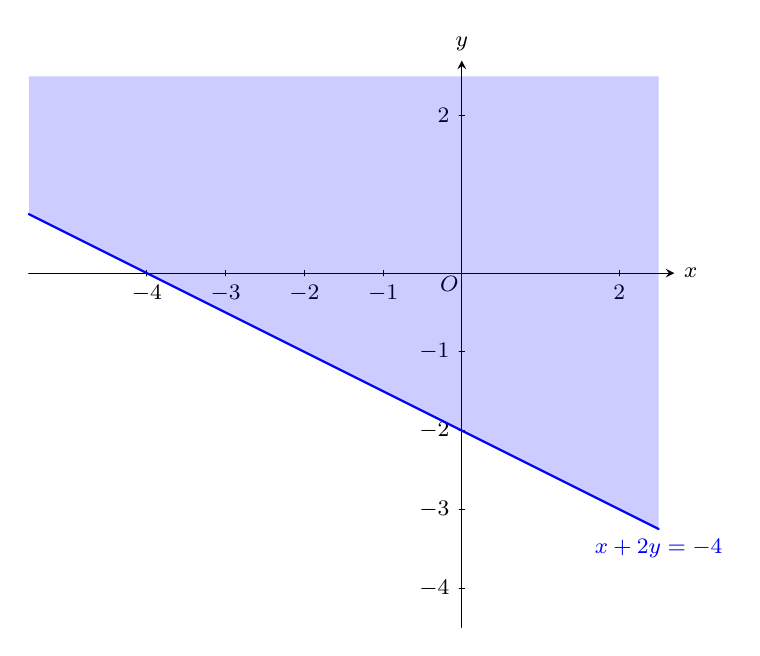
\begin{tikzpicture}[scale=1,font=\footnotesize,line join=round,line cap=round,>=stealth]
				\def\xmin{-5.5} \def\xmax{2.5}
				\def\ymin{-4.5} \def\ymax{2.5}
				\draw[->] (\xmin,0) -- (\xmax+0.2,0) node[right] {$x$};
				\draw[->] (0,\ymin) -- (0,\ymax+0.2) node[above] {$y$};
				\foreach \val in {-4,-3,-2,-1,2} {
					\draw (\val,1pt) -- (\val,-1pt) node[below] {$\val$};
					\ifnum\val=0\else\draw (1pt,\val) -- (-1pt,\val) node[left] {$\val$};\fi
				}
				\node[below left,inner sep=1pt] at (0,0) {$O$};
				\fill[blue, opacity=0.2] (\xmin, {-0.5*(\xmin)-2})-- plot[domain=\xmin:\xmax] (\x, {-0.5*(\x)-2})-- (\xmax, \ymax) -- (\xmin, \ymax) -- cycle;
				\draw[thick, blue, domain=\xmin:\xmax]
				plot (\x, {-0.5*(\x)-2}) node[below] {$x+2y=-4$};
			\end{tikzpicture}
		\end{center}
		Yêu cầu bài toán trở thành, tìm cặp $(x;y)$ sao cho $(x;y)$ thuộc miền tô đậm.
		\begin{itemize}
			\item Với $y=-1$, ta có $x\in\{-2;-1\}$.
			\item Với $y=-2$, không có giá trị $x$ nguyên âm thoả mãn.
		\end{itemize}
		Vậy có $2$ điểm $(-2;-1)$, $(-1;-1)$ thoả mãn bài toán.
	}
\end{ex}
\begin{ex}%[0D3V2-6]%[Dự án dề cương 3 Khối NH24-25-Đợt 2-Nguyễn Thanh Phong]
	Mỗi ngày Nga đều dành không quá 30 phút để đọc cả $2$ cuốn sách A, B. Nga đọc được $3$ trang sách A trong $2$ phút, đọc được $2$ trang sách B trong $1$ phút. Gọi $x$, $y$ lần lượt là số phút đọc sách A và số phút đọc sách B. Tìm điều kiện của $x$ và $y$ để Nga đọc được ít nhất $35$ trang sách trong một ngày.
	\loigiai{
		Gọi $x$, $y$ lần lượt là số phút đọc sách A và số phút đọc sách B trong một ngày $(x$, $y > 0)$. Tổng số phút đọc sách không quá $30$ phút nên $x + y \leq 30$.
		
		Số trang sách A đọc được sau $x$ phút là $\dfrac{3x}{2}$. Số trang sách B đọc được sau $y$ phút là $2y$.
		
		Nga đọc được ít nhất $35$ trang sách trong một ngày khi và chỉ khi $\dfrac{3x}{2} + 2y \geq 35$.
		
		Vậy $x$, $y$ cần thỏa mãn các điều kiện
		$
		\heva{
			&x > 0 \\
			&y > 0 \\
			&x + y \leq 30 \\
			&\dfrac{3x}{2} + 2y \geq 35.
		}
		$
	}
\end{ex}

\begin{ex}%[0D2V1-3]%[Dự án dề cương 3 Khối NH24-25-Đợt 2-Nguyễn Thanh Phong]
	Một rạp chiếu phim $2$D phục vụ khán giả một bộ phim mới với $2$ loại vé khác nhau. Vé loại $1$ (từ thứ $2$ đến thứ $5$) giá $80\,000$ đồng/vé, vé loại $2$ (từ thứ $6$ đến chủ nhật và ngày lễ) giá $100\,000$ đồng/vé. Để không phải bù lỗ thì số tiền vé thu được ở rạp chiếu phim này phải đạt tối thiểu $150$ triệu đồng. Hỏi số lượng vé bán được trong những trường hợp nào thì rạp chiếu phim phải bù lỗ?
	\loigiai{
		Gọi $x$, $y$ lần lượt là số vé loại $1$, loại $2$ bán được ($x$, $y \in \mathbb{N}$).\\
		Tổng số tiền bán vé là $80x + 100y$ nghìn đồng.\\
		Rạp chiếu phim phải bù lỗ trong trường hợp số tiền bán vé nhỏ hơn 150 triệu đồng, tức là
		\[80x + 100y < 15\,0000 \Rightarrow 4x + 5y < 7\,500. \quad  (1)\]
		Miền nghiệm của bất phương trình $(1)$ được xác định như sau\\
		\begin{itemize}
			\item Vẽ đường thẳng $d\colon 4x + 5y = 7\,500$.
			\item Chọn gốc tọa độ $O(0;0)$ và tính $4 \cdot 0 + 5 \cdot 0 < 7\,500$.
		\end{itemize}
		\begin{center}
			\begin{tikzpicture}[scale=1, font=\footnotesize, line join=round, line cap=round, >=stealth]
				\def\xmax{5} \def\ymax{5}
				\coordinate (A) at (4.5, 0);
				\coordinate (B) at (0, 3.5);
				\fill[pattern=north east lines, pattern color=gray!80]
				(B) -- (A) -- (\xmax, 0) -- (\xmax, \ymax) -- (0, \ymax) -- cycle;
				\draw[->] (-0.2,0) -- (\xmax+0.5,0) node[below] {$x$};
				\draw[->] (0,-0.2) -- (0,\ymax+0.5) node[left] {$y$};
				\draw[thick] (A) -- (B);
				\node[below left] at (0,0) {$O$};
				\node[above] at (A) {$A$};
				\node[below=2pt] at (A) {$1875$};
				\node[right] at (B) {$B$};
				\node[left=2pt] at (B) {$1500$};
			\end{tikzpicture}
		\end{center}
		Do đó miền nghiệm của bất phương trình $(1)$ là nửa mặt phẳng bờ $d$, chứa gốc tọa độ $O$, không kể đường thẳng $d$.\\
		Gọi $A$, $B$ lần lượt là giao điểm của $d$ và $Ox$, $Oy$. Khi đó, nếu bán được $x$ vé loại $1$ và $y$ vé loại $2$ mà điểm $(x; y)$ nằm trong miền tam giác $OAB$ không kể cạnh $AB$ thì rạp chiếu phim sẽ phải bù lỗ.
		
	}
\end{ex}